% Chapter 9: Prophet and TBATS for Multiple Seasonalities
% Modern approaches for complex seasonal patterns
% Bachelor program, Bucharest University of Economic Studies

\documentclass[9pt, aspectratio=169, t]{beamer}

% Ensure content fits on slides
\setbeamersize{text margin left=8mm, text margin right=8mm}

%=============================================================================
% THEME AND STYLE CONFIGURATION
%=============================================================================
\usetheme{Madrid}
\usecolortheme{seahorse}

% IDA-Inspired Color Palette
\definecolor{MainBlue}{RGB}{26, 58, 110}
\definecolor{AccentBlue}{RGB}{42, 82, 140}
\definecolor{IDAred}{RGB}{220, 53, 69}
\definecolor{DarkGray}{RGB}{51, 51, 51}
\definecolor{MediumGray}{RGB}{128, 128, 128}
\definecolor{LightGray}{RGB}{248, 248, 248}
\definecolor{VeryLightGray}{RGB}{235, 235, 235}
\definecolor{Crimson}{RGB}{220, 53, 69}
\definecolor{Forest}{RGB}{46, 125, 50}
\definecolor{Amber}{RGB}{181, 133, 63}
\definecolor{Orange}{RGB}{230, 126, 34}

\setbeamercolor{palette primary}{bg=MainBlue, fg=white}
\setbeamercolor{palette secondary}{bg=MainBlue!85, fg=white}
\setbeamercolor{palette tertiary}{bg=MainBlue!70, fg=white}
\setbeamercolor{structure}{fg=MainBlue}
\setbeamercolor{title}{fg=MainBlue}
\setbeamercolor{frametitle}{fg=MainBlue, bg=white}
\setbeamercolor{block title}{bg=MainBlue, fg=white}
\setbeamercolor{block body}{bg=VeryLightGray, fg=DarkGray}
\setbeamercolor{block title alerted}{bg=Crimson, fg=white}
\setbeamercolor{block body alerted}{bg=Crimson!8, fg=DarkGray}
\setbeamercolor{block title example}{bg=Forest, fg=white}
\setbeamercolor{block body example}{bg=Forest!8, fg=DarkGray}
\setbeamercolor{item}{fg=MainBlue}

\setbeamertemplate{navigation symbols}{}

\setbeamertemplate{footline}{
    \leavevmode%
    \hbox{%
        \begin{beamercolorbox}[wd=.333333\paperwidth,ht=2.5ex,dp=1ex,center]{author in head/foot}%
            \usebeamerfont{author in head/foot}\insertshortauthor
        \end{beamercolorbox}%
        \begin{beamercolorbox}[wd=.333333\paperwidth,ht=2.5ex,dp=1ex,center]{title in head/foot}%
            \usebeamerfont{title in head/foot}\insertshorttitle
        \end{beamercolorbox}%
        \begin{beamercolorbox}[wd=.333333\paperwidth,ht=2.5ex,dp=1ex,right]{date in head/foot}%
            \usebeamerfont{date in head/foot}\insertshortdate{}\hspace*{2em}
            \insertframenumber{} / \inserttotalframenumber\hspace*{2ex}
        \end{beamercolorbox}}%
    \vskip0pt%
}

%=============================================================================
% PACKAGES
%=============================================================================
\usepackage[utf8]{inputenc}
\usepackage[T1]{fontenc}
\usepackage{amsmath, amssymb, amsthm}
\usepackage{mathtools}
\usepackage{bm}
\usepackage{tikz}
\usetikzlibrary{arrows.meta, positioning, shapes, calc}
\usepackage{booktabs}
\usepackage{multirow}
\usepackage{array}
\usepackage{graphicx}
\usepackage{hyperref}
\hypersetup{colorlinks=false, pdfborder={0 0 0}}
\graphicspath{{logos/}{charts/}}

%=============================================================================
% THEOREM ENVIRONMENTS
%=============================================================================
\theoremstyle{definition}
\setbeamertemplate{theorems}[numbered]
\newtheorem{defn}{Definition}
\newtheorem{thm}{Theorem}
\newtheorem{prop}{Proposition}

%=============================================================================
% CUSTOM COMMANDS
%=============================================================================
\newcommand{\E}{\mathbb{E}}
\newcommand{\Var}{\text{Var}}
\newcommand{\Cov}{\text{Cov}}
\newcommand{\Corr}{\text{Corr}}
\newcommand{\R}{\mathbb{R}}

%=============================================================================
% TITLE INFORMATION
%=============================================================================
\title[Chapter 9: Prophet \& TBATS]{Chapter 9: Prophet and TBATS}
\subtitle{Modern Models for Multiple Seasonalities}
\author[D. Pele]{Daniel Pele, PhD}
\institute[ASE]{Bucharest University of Economic Studies\\Faculty of Cybernetics, Statistics and Economic Informatics}
\date{2025-2026}

\begin{document}

%=============================================================================
% TITLE SLIDE
%=============================================================================
\begin{frame}
    \titlepage
\end{frame}

%=============================================================================
% OUTLINE
%=============================================================================
\begin{frame}{Outline}
    \tableofcontents
\end{frame}

%=============================================================================
% SECTION 1: MOTIVATION
%=============================================================================
\section{Multiple Seasonalities}

\begin{frame}{The Problem: Complex Seasonal Patterns}
    \begin{block}{Real-World Examples}
        \begin{itemize}
            \item \textbf{Hourly electricity demand}: Daily + Weekly + Annual patterns
            \item \textbf{Website traffic}: Daily + Weekly + Holiday effects
            \item \textbf{Retail sales}: Weekly + Monthly + Annual + Holiday effects
            \item \textbf{Call center volume}: Hourly + Daily + Weekly patterns
        \end{itemize}
    \end{block}

    \vspace{0.3cm}

    \begin{alertblock}{SARIMA Limitation}
        Standard SARIMA$(p,d,q)(P,D,Q)_s$ handles only \textbf{one} seasonal period $s$.

        \vspace{0.2cm}
        For hourly data with daily AND weekly patterns, we need $s_1 = 24$ and $s_2 = 168$.
    \end{alertblock}
\end{frame}

\begin{frame}{Solutions for Multiple Seasonalities}
    \begin{columns}[T]
        \column{0.5\textwidth}
        \begin{block}{Traditional Approaches}
            \begin{itemize}
                \item \textbf{Fourier terms}: Add sin/cos regressors
                \item \textbf{Dummy variables}: Many parameters
                \item \textbf{Nested models}: Complex specification
            \end{itemize}
        \end{block}

        \column{0.5\textwidth}
        \begin{exampleblock}{Modern Approaches}
            \begin{itemize}
                \item \textbf{TBATS}: Automatic, handles many periods
                \item \textbf{Prophet}: Flexible, interpretable
                \item \textbf{Neural methods}: Deep learning
            \end{itemize}
        \end{exampleblock}
    \end{columns}

    \vspace{0.5cm}

    \begin{center}
        \begin{tabular}{lcc}
            \toprule
            \textbf{Method} & \textbf{Max Seasonalities} & \textbf{Interpretable} \\
            \midrule
            SARIMA & 1 & Yes \\
            Fourier + ARIMA & Multiple & Moderate \\
            TBATS & Multiple & Moderate \\
            Prophet & Multiple & Yes \\
            \bottomrule
        \end{tabular}
    \end{center}
\end{frame}

%=============================================================================
% SECTION 2: TBATS
%=============================================================================
\section{TBATS Model}

\begin{frame}{TBATS: What Does It Stand For?}
    \begin{block}{TBATS Components}
        \begin{description}
            \item[T] \textbf{Trigonometric} seasonality using Fourier terms
            \item[B] \textbf{Box-Cox} transformation for variance stabilization
            \item[A] \textbf{ARMA} errors for remaining autocorrelation
            \item[T] \textbf{Trend} component (possibly damped)
            \item[S] \textbf{Seasonal} components (multiple allowed)
        \end{description}
    \end{block}

    \vspace{0.3cm}

    \begin{exampleblock}{Key Innovation}
        TBATS uses \textbf{trigonometric representation} of seasonality:
        \[
        s_t^{(i)} = \sum_{j=1}^{k_i} \left[ s_j^{(i)} \cos\left(\frac{2\pi j t}{m_i}\right) + s_j^{*(i)} \sin\left(\frac{2\pi j t}{m_i}\right) \right]
        \]
        where $m_i$ is the $i$-th seasonal period and $k_i$ is the number of harmonics.
    \end{exampleblock}
\end{frame}

\begin{frame}{TBATS Model Structure}
    \begin{block}{Full Model Specification}
        \begin{align}
            y_t^{(\omega)} &= \ell_{t-1} + \phi b_{t-1} + \sum_{i=1}^{T} s_{t-m_i}^{(i)} + d_t \\[0.3cm]
            \ell_t &= \ell_{t-1} + \phi b_{t-1} + \alpha d_t \\[0.2cm]
            b_t &= \phi b_{t-1} + \beta d_t \\[0.2cm]
            d_t &= \sum_{i=1}^{p} \varphi_i d_{t-i} + \sum_{j=1}^{q} \theta_j \varepsilon_{t-j} + \varepsilon_t
        \end{align}
    \end{block}

    \vspace{0.2cm}

    {\small
    Where:
    \begin{itemize}
        \item $y_t^{(\omega)}$ is Box-Cox transformed series (if $\omega \neq 1$)
        \item $\ell_t$ is local level, $b_t$ is trend with damping $\phi$
        \item $s_t^{(i)}$ are $T$ seasonal components with periods $m_1, \ldots, m_T$
        \item $d_t$ is ARMA$(p,q)$ error process
    \end{itemize}
    }
\end{frame}

\begin{frame}{TBATS: Trigonometric Seasonality}
    \begin{block}{Why Fourier/Trigonometric Terms?}
        \begin{enumerate}
            \item \textbf{Parsimonious}: Fewer parameters than dummy variables
            \item \textbf{Smooth}: Captures smooth seasonal patterns naturally
            \item \textbf{Flexible}: Number of harmonics $k$ controls complexity
            \item \textbf{Non-integer periods}: Can handle $s = 365.25$ for daily data
        \end{enumerate}
    \end{block}

    \vspace{0.3cm}

    \begin{columns}[T]
        \column{0.5\textwidth}
        \begin{exampleblock}{Low $k$ (few harmonics)}
            \begin{itemize}
                \item Smooth pattern
                \item Fewer parameters
                \item May miss sharp peaks
            \end{itemize}
        \end{exampleblock}

        \column{0.5\textwidth}
        \begin{alertblock}{High $k$ (many harmonics)}
            \begin{itemize}
                \item Can capture any pattern
                \item More parameters
                \item Risk of overfitting
            \end{itemize}
        \end{alertblock}
    \end{columns}
\end{frame}

\begin{frame}{TBATS in Practice}
    \begin{block}{Python Implementation}
        \texttt{tbats} package provides automatic model selection:
        \begin{itemize}
            \item Automatically selects Box-Cox parameter $\omega$
            \item Chooses number of harmonics $k_i$ for each seasonal period
            \item Selects ARMA orders $(p,q)$
            \item Tests damped vs non-damped trend
        \end{itemize}
    \end{block}

    \vspace{0.3cm}

    \begin{exampleblock}{Code Example}
        \small
        \texttt{from tbats import TBATS}\\
        \texttt{estimator = TBATS(seasonal\_periods=[7, 365.25])}\\
        \texttt{model = estimator.fit(y)}\\
        \texttt{forecast = model.forecast(steps=30)}
    \end{exampleblock}

    \vspace{0.2cm}

    {\small \textbf{Note}: BATS is the simpler version without trigonometric terms (uses traditional seasonal states).}
\end{frame}

\begin{frame}{TBATS: Advantages and Limitations}
    \begin{columns}[T]
        \column{0.5\textwidth}
        \begin{exampleblock}{Advantages}
            \begin{itemize}
                \item Handles \textbf{multiple} seasonal periods
                \item \textbf{Automatic} model selection
                \item Handles \textbf{non-integer} periods (365.25)
                \item \textbf{Box-Cox} for heteroskedasticity
                \item Good for \textbf{high-frequency} data
            \end{itemize}
        \end{exampleblock}

        \column{0.5\textwidth}
        \begin{alertblock}{Limitations}
            \begin{itemize}
                \item \textbf{Computationally intensive}
                \item No \textbf{external regressors}
                \item Less \textbf{interpretable} than Prophet
                \item Can be \textbf{slow} for very long series
                \item Requires \textbf{sufficient data} per season
            \end{itemize}
        \end{alertblock}
    \end{columns}
\end{frame}

%=============================================================================
% SECTION 3: PROPHET
%=============================================================================
\section{Facebook Prophet}

\begin{frame}{Prophet: Overview}
    \begin{block}{What is Prophet?}
        Prophet is a forecasting procedure developed by Facebook (Meta) in 2017.

        \vspace{0.2cm}

        Designed for \textbf{business time series} with:
        \begin{itemize}
            \item Strong seasonal effects (daily, weekly, yearly)
            \item Holiday effects
            \item Trend changes (changepoints)
            \item Missing data and outliers
        \end{itemize}
    \end{block}

    \vspace{0.3cm}

    \begin{exampleblock}{Key Philosophy}
        \begin{center}
            \textit{``Analyst-in-the-loop'' forecasting}
        \end{center}
        Prophet is designed to be tuned by analysts who have domain knowledge but may not be time series experts.
    \end{exampleblock}
\end{frame}

\begin{frame}{Prophet Model Structure}
    \begin{block}{Decomposition Approach}
        Prophet uses an \textbf{additive decomposition}:
        \[
        y(t) = g(t) + s(t) + h(t) + \varepsilon_t
        \]
    \end{block}

    \vspace{0.3cm}

    \begin{columns}[T]
        \column{0.33\textwidth}
        \begin{block}{$g(t)$: Trend}
            \begin{itemize}
                \item Linear or logistic
                \item Automatic changepoints
                \item Growth saturation
            \end{itemize}
        \end{block}

        \column{0.33\textwidth}
        \begin{block}{$s(t)$: Seasonality}
            \begin{itemize}
                \item Fourier series
                \item Multiple periods
                \item Custom seasonality
            \end{itemize}
        \end{block}

        \column{0.33\textwidth}
        \begin{block}{$h(t)$: Holidays}
            \begin{itemize}
                \item Country holidays
                \item Custom events
                \item Window effects
            \end{itemize}
        \end{block}
    \end{columns}
\end{frame}

\begin{frame}{Prophet: Trend Component}
    \begin{block}{Linear Trend with Changepoints}
        \[
        g(t) = (k + \bm{a}(t)^T \bm{\delta}) \cdot t + (m + \bm{a}(t)^T \bm{\gamma})
        \]
        where:
        \begin{itemize}
            \item $k$ is the base growth rate
            \item $\bm{\delta}$ is a vector of rate adjustments at changepoints
            \item $\bm{a}(t)$ indicates which changepoints are active at time $t$
            \item $m$ is the offset, $\bm{\gamma}$ ensures continuity
        \end{itemize}
    \end{block}

    \vspace{0.3cm}

    \begin{exampleblock}{Logistic Growth (for saturating trends)}
        \[
        g(t) = \frac{C(t)}{1 + \exp(-(k + \bm{a}(t)^T \bm{\delta})(t - (m + \bm{a}(t)^T \bm{\gamma})))}
        \]
        where $C(t)$ is the (possibly time-varying) carrying capacity.
    \end{exampleblock}
\end{frame}

\begin{frame}{Prophet: Seasonality Component}
    \begin{block}{Fourier Series Representation}
        For a seasonal period $P$, Prophet uses:
        \[
        s(t) = \sum_{n=1}^{N} \left[ a_n \cos\left(\frac{2\pi n t}{P}\right) + b_n \sin\left(\frac{2\pi n t}{P}\right) \right]
        \]
    \end{block}

    \vspace{0.3cm}

    \begin{exampleblock}{Default Settings}
        \begin{center}
        \begin{tabular}{lcc}
            \toprule
            \textbf{Seasonality} & \textbf{Period} & \textbf{Fourier Order} \\
            \midrule
            Yearly & 365.25 days & 10 \\
            Weekly & 7 days & 3 \\
            Daily & 1 day & 4 \\
            \bottomrule
        \end{tabular}
        \end{center}
    \end{exampleblock}

    \vspace{0.2cm}

    {\small Higher Fourier order $N$ = more flexibility (can fit more complex patterns) but higher risk of overfitting.}
\end{frame}

\begin{frame}{Prophet: Holiday Effects}
    \begin{block}{Holiday Model}
        \[
        h(t) = Z(t) \cdot \bm{\kappa}
        \]
        where $Z(t)$ is an indicator matrix for holidays and $\bm{\kappa}$ are holiday effects.
    \end{block}

    \vspace{0.3cm}

    \begin{exampleblock}{Features}
        \begin{itemize}
            \item \textbf{Built-in holidays}: 60+ countries supported
            \item \textbf{Custom holidays}: Add your own events (Black Friday, company events)
            \item \textbf{Window effects}: Holidays can affect days before/after
            \item \textbf{Prior scale}: Control regularization of holiday effects
        \end{itemize}
    \end{exampleblock}

    \vspace{0.3cm}

    \begin{block}{Code Example}
        \small
        \texttt{holidays = pd.DataFrame(\{'holiday': 'black\_friday', ....\})}\\
        \texttt{model = Prophet(holidays=holidays)}
    \end{block}
\end{frame}

\begin{frame}{Prophet in Practice}
    \begin{block}{Basic Usage}
        \small
        \texttt{from prophet import Prophet}\\
        \texttt{import pandas as pd}\\[0.2cm]
        \texttt{\# Data must have columns 'ds' (date) and 'y' (value)}\\
        \texttt{df = pd.DataFrame(\{'ds': dates, 'y': values\})}\\[0.2cm]
        \texttt{model = Prophet()}\\
        \texttt{model.fit(df)}\\[0.2cm]
        \texttt{future = model.make\_future\_dataframe(periods=365)}\\
        \texttt{forecast = model.predict(future)}
    \end{block}

    \vspace{0.3cm}

    \begin{exampleblock}{Adding Custom Seasonality}
        \small
        \texttt{model = Prophet(weekly\_seasonality=False)}\\
        \texttt{model.add\_seasonality(name='monthly', period=30.5, fourier\_order=5)}\\
        \texttt{model.add\_seasonality(name='quarterly', period=91.25, fourier\_order=3)}
    \end{exampleblock}
\end{frame}

\begin{frame}{Prophet: Uncertainty Quantification}
    \begin{block}{Three Sources of Uncertainty}
        \begin{enumerate}
            \item \textbf{Trend uncertainty}: Future changepoints are uncertain
            \item \textbf{Seasonality uncertainty}: Parameter estimation uncertainty
            \item \textbf{Observation noise}: Inherent randomness
        \end{enumerate}
    \end{block}

    \vspace{0.3cm}

    \begin{columns}[T]
        \column{0.6\textwidth}
        \begin{exampleblock}{Prediction Intervals}
            Prophet provides:
            \begin{itemize}
                \item Point forecast: \texttt{yhat}
                \item Lower bound: \texttt{yhat\_lower}
                \item Upper bound: \texttt{yhat\_upper}
            \end{itemize}

            \vspace{0.2cm}

            Default is 80\% interval.\\
            Change with \texttt{interval\_width=0.95}
        \end{exampleblock}

        \column{0.4\textwidth}
        \begin{alertblock}{Note}
            Uncertainty grows with forecast horizon, especially for trend uncertainty.
        \end{alertblock}
    \end{columns}
\end{frame}

\begin{frame}{Prophet: Tuning Parameters}
    \begin{block}{Key Parameters}
        \begin{center}
        \small
        \begin{tabular}{p{4cm}p{8cm}}
            \toprule
            \textbf{Parameter} & \textbf{Effect} \\
            \midrule
            \texttt{changepoint\_prior\_scale} & Trend flexibility (default: 0.05) \\
            \texttt{seasonality\_prior\_scale} & Seasonality flexibility (default: 10) \\
            \texttt{holidays\_prior\_scale} & Holiday effect size (default: 10) \\
            \texttt{seasonality\_mode} & 'additive' or 'multiplicative' \\
            \texttt{changepoint\_range} & Portion of history for changepoints \\
            \bottomrule
        \end{tabular}
        \end{center}
    \end{block}

    \vspace{0.3cm}

    \begin{exampleblock}{Practical Tips}
        \begin{itemize}
            \item \textbf{Overfitting trend?} Decrease \texttt{changepoint\_prior\_scale}
            \item \textbf{Underfitting seasonality?} Increase \texttt{seasonality\_prior\_scale}
            \item \textbf{Seasonal amplitude varies?} Use \texttt{seasonality\_mode='multiplicative'}
        \end{itemize}
    \end{exampleblock}
\end{frame}

\begin{frame}{Prophet: Advantages and Limitations}
    \begin{columns}[T]
        \column{0.5\textwidth}
        \begin{exampleblock}{Advantages}
            \begin{itemize}
                \item \textbf{Easy to use}: Minimal tuning needed
                \item \textbf{Interpretable}: Clear decomposition
                \item \textbf{Handles missing data} well
                \item \textbf{Holiday effects} built-in
                \item \textbf{Multiple seasonalities}
                \item \textbf{External regressors} supported
                \item \textbf{Fast} fitting
            \end{itemize}
        \end{exampleblock}

        \column{0.5\textwidth}
        \begin{alertblock}{Limitations}
            \begin{itemize}
                \item \textbf{Not ARIMA-based}: No autocorrelation modeling
                \item \textbf{Daily data focus}: Less suited for very high frequency
                \item \textbf{Trend assumptions}: Linear/logistic may not fit
                \item \textbf{No built-in CV}: Must implement manually
                \item \textbf{Overfitting risk} with many seasonalities
            \end{itemize}
        \end{alertblock}
    \end{columns}
\end{frame}

%=============================================================================
% SECTION 4: COMPARISON
%=============================================================================
\section{Comparison and Guidelines}

\begin{frame}{TBATS vs Prophet: Head-to-Head}
    \begin{center}
    \small
    \begin{tabular}{p{4cm}p{4.5cm}p{4.5cm}}
        \toprule
        \textbf{Feature} & \textbf{TBATS} & \textbf{Prophet} \\
        \midrule
        Multiple seasonalities & Yes (automatic) & Yes (manual or auto) \\
        Holiday effects & No & Yes (built-in) \\
        External regressors & No & Yes \\
        Trend changepoints & No (smooth) & Yes (automatic) \\
        Missing data & Interpolation needed & Handles natively \\
        Interpretability & Moderate & High \\
        Computation speed & Slow & Fast \\
        High-frequency data & Good & Moderate \\
        Non-integer periods & Yes (e.g., 365.25) & Yes \\
        Uncertainty intervals & Yes & Yes \\
        \bottomrule
    \end{tabular}
    \end{center}
\end{frame}

\begin{frame}{When to Use Each Model}
    \begin{columns}[T]
        \column{0.5\textwidth}
        \begin{block}{Use TBATS when:}
            \begin{itemize}
                \item High-frequency data (hourly, sub-daily)
                \item Multiple complex seasonal periods
                \item No external regressors needed
                \item Automatic model selection preferred
                \item Traditional state-space framework desired
            \end{itemize}
        \end{block}

        \column{0.5\textwidth}
        \begin{block}{Use Prophet when:}
            \begin{itemize}
                \item Business forecasting (daily/weekly)
                \item Holiday effects are important
                \item Trend has structural breaks
                \item Missing data present
                \item Interpretability is key
                \item External regressors available
            \end{itemize}
        \end{block}
    \end{columns}

    \vspace{0.5cm}

    \begin{exampleblock}{General Guideline}
        \begin{center}
            \textbf{Prophet} for business applications with daily data\\
            \textbf{TBATS} for technical applications with high-frequency data
        \end{center}
    \end{exampleblock}
\end{frame}

\begin{frame}{Decision Flowchart}
    \begin{center}
    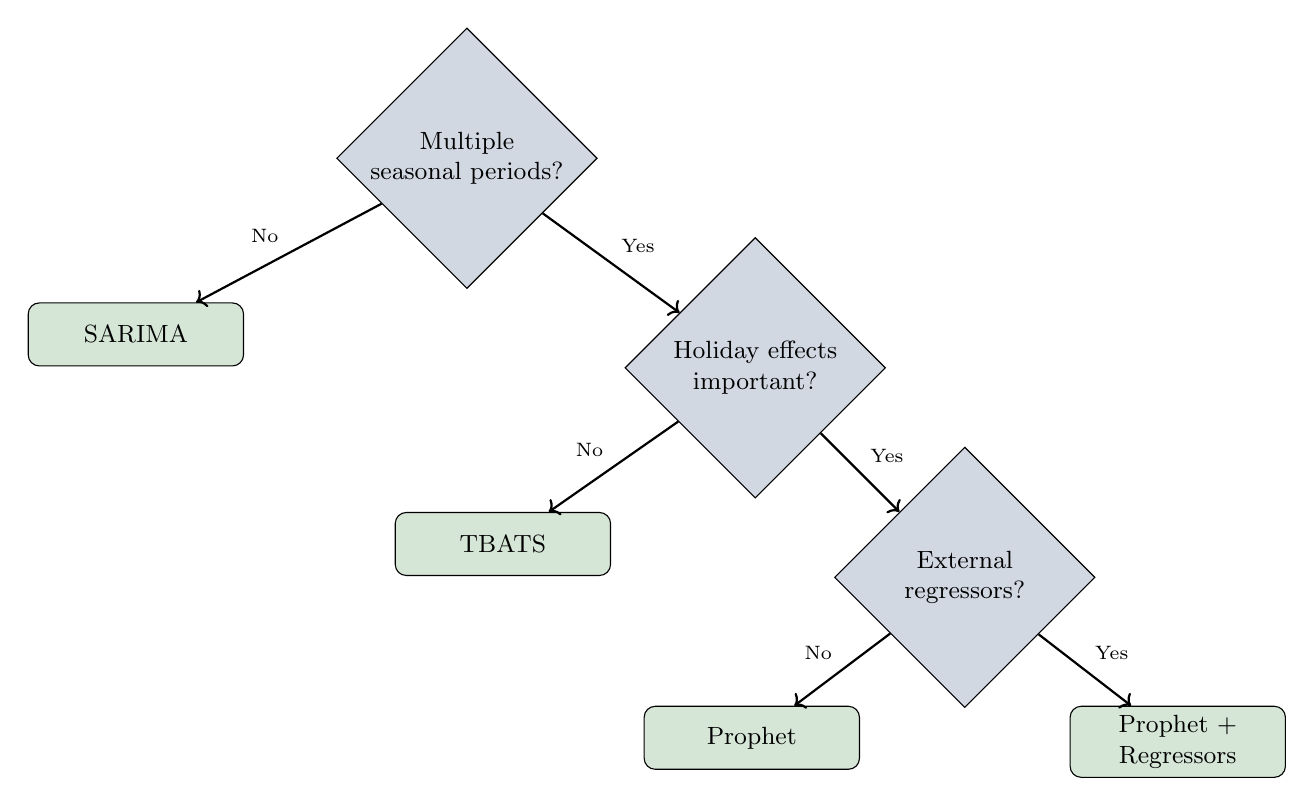
\begin{tikzpicture}[
        node distance=1.2cm,
        decision/.style={diamond, draw, fill=MainBlue!20, text width=2.5cm, text centered, inner sep=1pt, font=\small},
        block/.style={rectangle, draw, fill=Forest!20, text width=2.5cm, text centered, rounded corners, minimum height=0.8cm, font=\small},
        line/.style={draw, ->, thick}
    ]
        \node [decision] (q1) {Multiple seasonal periods?};
        \node [block, below left=1cm and 2cm of q1] (sarima) {SARIMA};
        \node [decision, below right=1cm and 2cm of q1] (q2) {Holiday effects important?};
        \node [block, below left=1cm and 1cm of q2] (tbats) {TBATS};
        \node [decision, below right=1cm and 1cm of q2] (q3) {External regressors?};
        \node [block, below left=0.8cm and 0.5cm of q3] (prophet1) {Prophet};
        \node [block, below right=0.8cm and 0.5cm of q3] (prophet2) {Prophet + Regressors};

        \path [line] (q1) -- node[above left, font=\scriptsize] {No} (sarima);
        \path [line] (q1) -- node[above right, font=\scriptsize] {Yes} (q2);
        \path [line] (q2) -- node[above left, font=\scriptsize] {No} (tbats);
        \path [line] (q2) -- node[above right, font=\scriptsize] {Yes} (q3);
        \path [line] (q3) -- node[above left, font=\scriptsize] {No} (prophet1);
        \path [line] (q3) -- node[above right, font=\scriptsize] {Yes} (prophet2);
    \end{tikzpicture}
    \end{center}
\end{frame}

%=============================================================================
% SECTION 5: PRACTICAL EXAMPLE
%=============================================================================
\section{Case Study}

\begin{frame}{Case Study: Energy Demand Forecasting}
    \begin{block}{Problem}
        Forecast hourly electricity demand with:
        \begin{itemize}
            \item \textbf{Daily pattern}: Peak at noon and evening
            \item \textbf{Weekly pattern}: Lower on weekends
            \item \textbf{Annual pattern}: Higher in summer (AC) and winter (heating)
            \item \textbf{Holiday effects}: Lower demand on holidays
        \end{itemize}
    \end{block}

    \vspace{0.3cm}

    \begin{exampleblock}{Approach}
        \begin{enumerate}
            \item Try TBATS with periods [24, 168, 8766]
            \item Try Prophet with daily, weekly, yearly seasonality + holidays
            \item Compare using cross-validation
        \end{enumerate}
    \end{exampleblock}
\end{frame}

\begin{frame}{Case Study: Results Interpretation}
    \begin{block}{Evaluation Metrics}
        \begin{itemize}
            \item \textbf{MAPE}: Mean Absolute Percentage Error
            \item \textbf{RMSE}: Root Mean Square Error
            \item \textbf{Coverage}: \% of actuals within prediction interval
        \end{itemize}
    \end{block}

    \vspace{0.3cm}

    \begin{exampleblock}{Typical Findings}
        \begin{center}
        \begin{tabular}{lccc}
            \toprule
            \textbf{Model} & \textbf{MAPE} & \textbf{RMSE} & \textbf{Coverage} \\
            \midrule
            SARIMA (daily only) & 8.5\% & 450 MW & 75\% \\
            TBATS & 4.2\% & 220 MW & 82\% \\
            Prophet & 4.8\% & 250 MW & 85\% \\
            Prophet + holidays & 3.9\% & 200 MW & 88\% \\
            \bottomrule
        \end{tabular}
        \end{center}
    \end{exampleblock}

    {\small Multiple seasonality models significantly outperform single-seasonality SARIMA.}
\end{frame}

%=============================================================================
% SECTION 6: SUMMARY
%=============================================================================
\section{Summary}

\begin{frame}{Key Takeaways}
    \begin{block}{Multiple Seasonalities}
        \begin{itemize}
            \item Real-world data often has multiple seasonal patterns
            \item Standard SARIMA handles only one seasonal period
            \item TBATS and Prophet are designed for this challenge
        \end{itemize}
    \end{block}

    \vspace{0.3cm}

    \begin{exampleblock}{Model Selection}
        \begin{itemize}
            \item \textbf{TBATS}: Automatic, handles high-frequency, no external regressors
            \item \textbf{Prophet}: Interpretable, holiday effects, external regressors
            \item Both use Fourier terms for efficient seasonality representation
        \end{itemize}
    \end{exampleblock}

    \vspace{0.3cm}

    \begin{alertblock}{Remember}
        Always validate with proper time series cross-validation!
    \end{alertblock}
\end{frame}

\begin{frame}{Questions?}
    \begin{center}
        \Large\textcolor{MainBlue}{Questions?}

        \vspace{1cm}

        \normalsize
        \textbf{Next Steps:}
        \begin{itemize}
            \item Practice with the Jupyter notebook
            \item Try Prophet on your own data
            \item Explore NeuralProphet for deep learning extension
        \end{itemize}
    \end{center}
\end{frame}

\end{document}
